\documentclass[12pt,ngerman,compress]{beamer}
\usepackage[ngerman]{babel}
\usepackage[utf8]{inputenc}
\usepackage{graphicx}

\usepackage[protrusion=true,expansion=false]{microtype}

\title[Python for Kids]{\large Monty und Python werden Hacker}
\author[Carina Willbold]{\small Carina Willbold \\ $\heartsuit$ WIP Projekt für Kinder $\heartsuit$ \\ \vspace*{1 cm}\small{Zusammenarbeit mit Ingo Blechschmidt}}
\institute[Universität Augsburg]{}
\date{%\includegraphics[scale = 0.4]{meme.jpg} \\ 
\vspace{1em} 13. Juni 2015 \\ Tübinger Linux-Infotag \\  }

%\usetheme[secheader]{Madrid}  %Warsaw
\usetheme{Antibes}
%\usecolortheme[RGB={0,101,97}]{structure}
\useoutertheme{split}
\usecolortheme{orchid}
\usefonttheme{serif}
%\usepackage{palatino}
\usepackage[T1]{fontenc}
\usepackage{libertine}
\useinnertheme{rectangles}
\setbeamertemplate{frametitle}[default][center]
\linespread{1.1}
%\setbeamercovered{transparent}
%\usepackage{lmodern}
%\usepackage{bookman}

\setbeamertemplate{navigation symbols}{}
\setbeamertemplate{headline}{}

\newcommand*\oldmacroB{}%
\let\oldmacroB\insertshorttitle%
\renewcommand*\insertshorttitle{%
        \oldmacroB\hfill%
  \insertframenumber\,/\,\inserttotalframenumber\hfill}

\newcommand{\dashdash}{{\usebeamercolor[fg]{itemize item}--{}}}
\definecolor{darkgreen}{RGB}{0,100,0}
\definecolor{darkred}{RGB}{139,0,0}
\newlength\figureheight
    \newlength\figurewidth
\begin{document}

\frame{\titlepage}

%\frame[t]{\frametitle{Outline}\tableofcontents}





%\frame[t]{\frametitle{Navier--Stokes equation}
%\begin{picture}(300,0)\linethickness{0.5mm}
%\put(20,-85){\makebox(325,100){\centering\tabular{@{}l@{}}$
%       \rho\frac{\partial\T{v}}{\partial t} - \nu\Delta\T{v} + \rho (\T{v} \cdot \nabla) \T{v} + \nabla p = \T{F} \hspace{5 mm}\quad\text{in}\quad \Omega \times (0,T)$\\
%	  $\quad\quad\quad\quad\quad\quad\quad\quad\quad\quad\hspace{1.9 mm}\nabla\cdot\T{v} = 0 \hspace{5 mm}\quad\text{in}\quad\Omega\times (0,T)$\\
%	  $\quad\quad\quad\quad\quad\quad\quad\quad\quad\quad\hspace{8.4 mm}\T{v} = \T{v}_{\text{in}}\hspace{1.5 mm}\quad \text{on}\quad\color{red}{\Gamma_{\text{in}}\times(0,T),$\\
%	  $\quad\quad\quad\quad\quad\quad\quad\quad\quad\quad\hspace{8.4 mm}\T{v} = 0 \hspace{ 5 mm}\quad\text{on}\quad\Gamma_{\text{lat}}\times(0,T)$\\
%	  $\quad\quad\quad\quad\quad\quad\hspace{7.2 mm}\nu\frac{\partial \T{v}}{\partial \T{n}_\Gamma} - p\T{n}_{\Gamma} = 0\hspace{5 mm}\quad \text{on}\quad\color{blue}{\Gamma_{\text{out}}}\times(0,T)$\\
%	  $\quad\quad\quad\quad\quad\quad\quad\quad\quad\hspace{4.2 mm}\T{v}(\cdot,0) = \T{v}_{0} \hspace{3 mm}\quad\text{in}\quad\Omega
 %      $\endtabular}}
% \put(30,-180){\color{blue}\line(1,0){240}}\put(30,-180){\line(0,1){80}}\put(270,-180){\line(0,1){80}}\put(30,-150){\color{gray}\line(1,0){240}}
%    \put(45,-100){\color{red}\line(1,0){25}} \put(30,-100){\line(1,0){15}}\put(70,-100){\line(1,0){160}}\put(230,-100){\color{red}\line(1,0){25}}\put(255,-100){\line(1,0){15}}
%    \put(45,-105){\color{red}\line(0,1){10}}\put(70,-105){\color{red}\line(0,1){10}}\put(230,-105){\color{red}\line(0,1){10}}\put(255,-105){\color{red}\line(0,1){10}}\put(140,-176){\makebox(20,20){$\Omega_{2}$}}\put(140,-135){\makebox(20,20){$\Omega_{1}$}}
%\end{picture}
%}

\frame[t]{\frametitle{Idee und Konzept}
\begin{itemize}
 \item Sachbuch für Kinder um Python zu lernen
 \item Motivation: Kinder möglichst früh ans Programmieren heranführen
 \item Kein trockener Sachbuchstil
 \item Fantasiegeschichte zum Mitlernen 
 \item In jedem Kapitel eine Herausforderung am Ende, die 
       zu einem größeren Porjekt führt
 \item Ziel: Kind sollte am Ende z.B. ein Spiel geschrieben haben       
\end{itemize}


}

% \frame[t]{\frametitle{Die Idee für die Geschichte}
% \begin{itemize}
%  \item Protagonistin wird von Aliens entführt, deren Mutterschiff nicht mehr funktioniert
%  \item Eigener Programmierer ist verschollen -> Protagonistin soll Python lernen und das Schiff reparieren
%  \item In jedem Kapitel wird ein Konzept vorgestellt (z.B. Schleifen)
%  \item Kapitel werden von vielen Übungsaufgaben begleitet
%  \item Finale Aufgabe am Ende der Kapitel, die Fortschritt in der Reperatur für die   
%        Protagonistin bedeutet und für den Leser Fortschritt in einem kleinen Miniprojekt
% \end{itemize}
% 
% }


\frame[t]{
\begin{center}
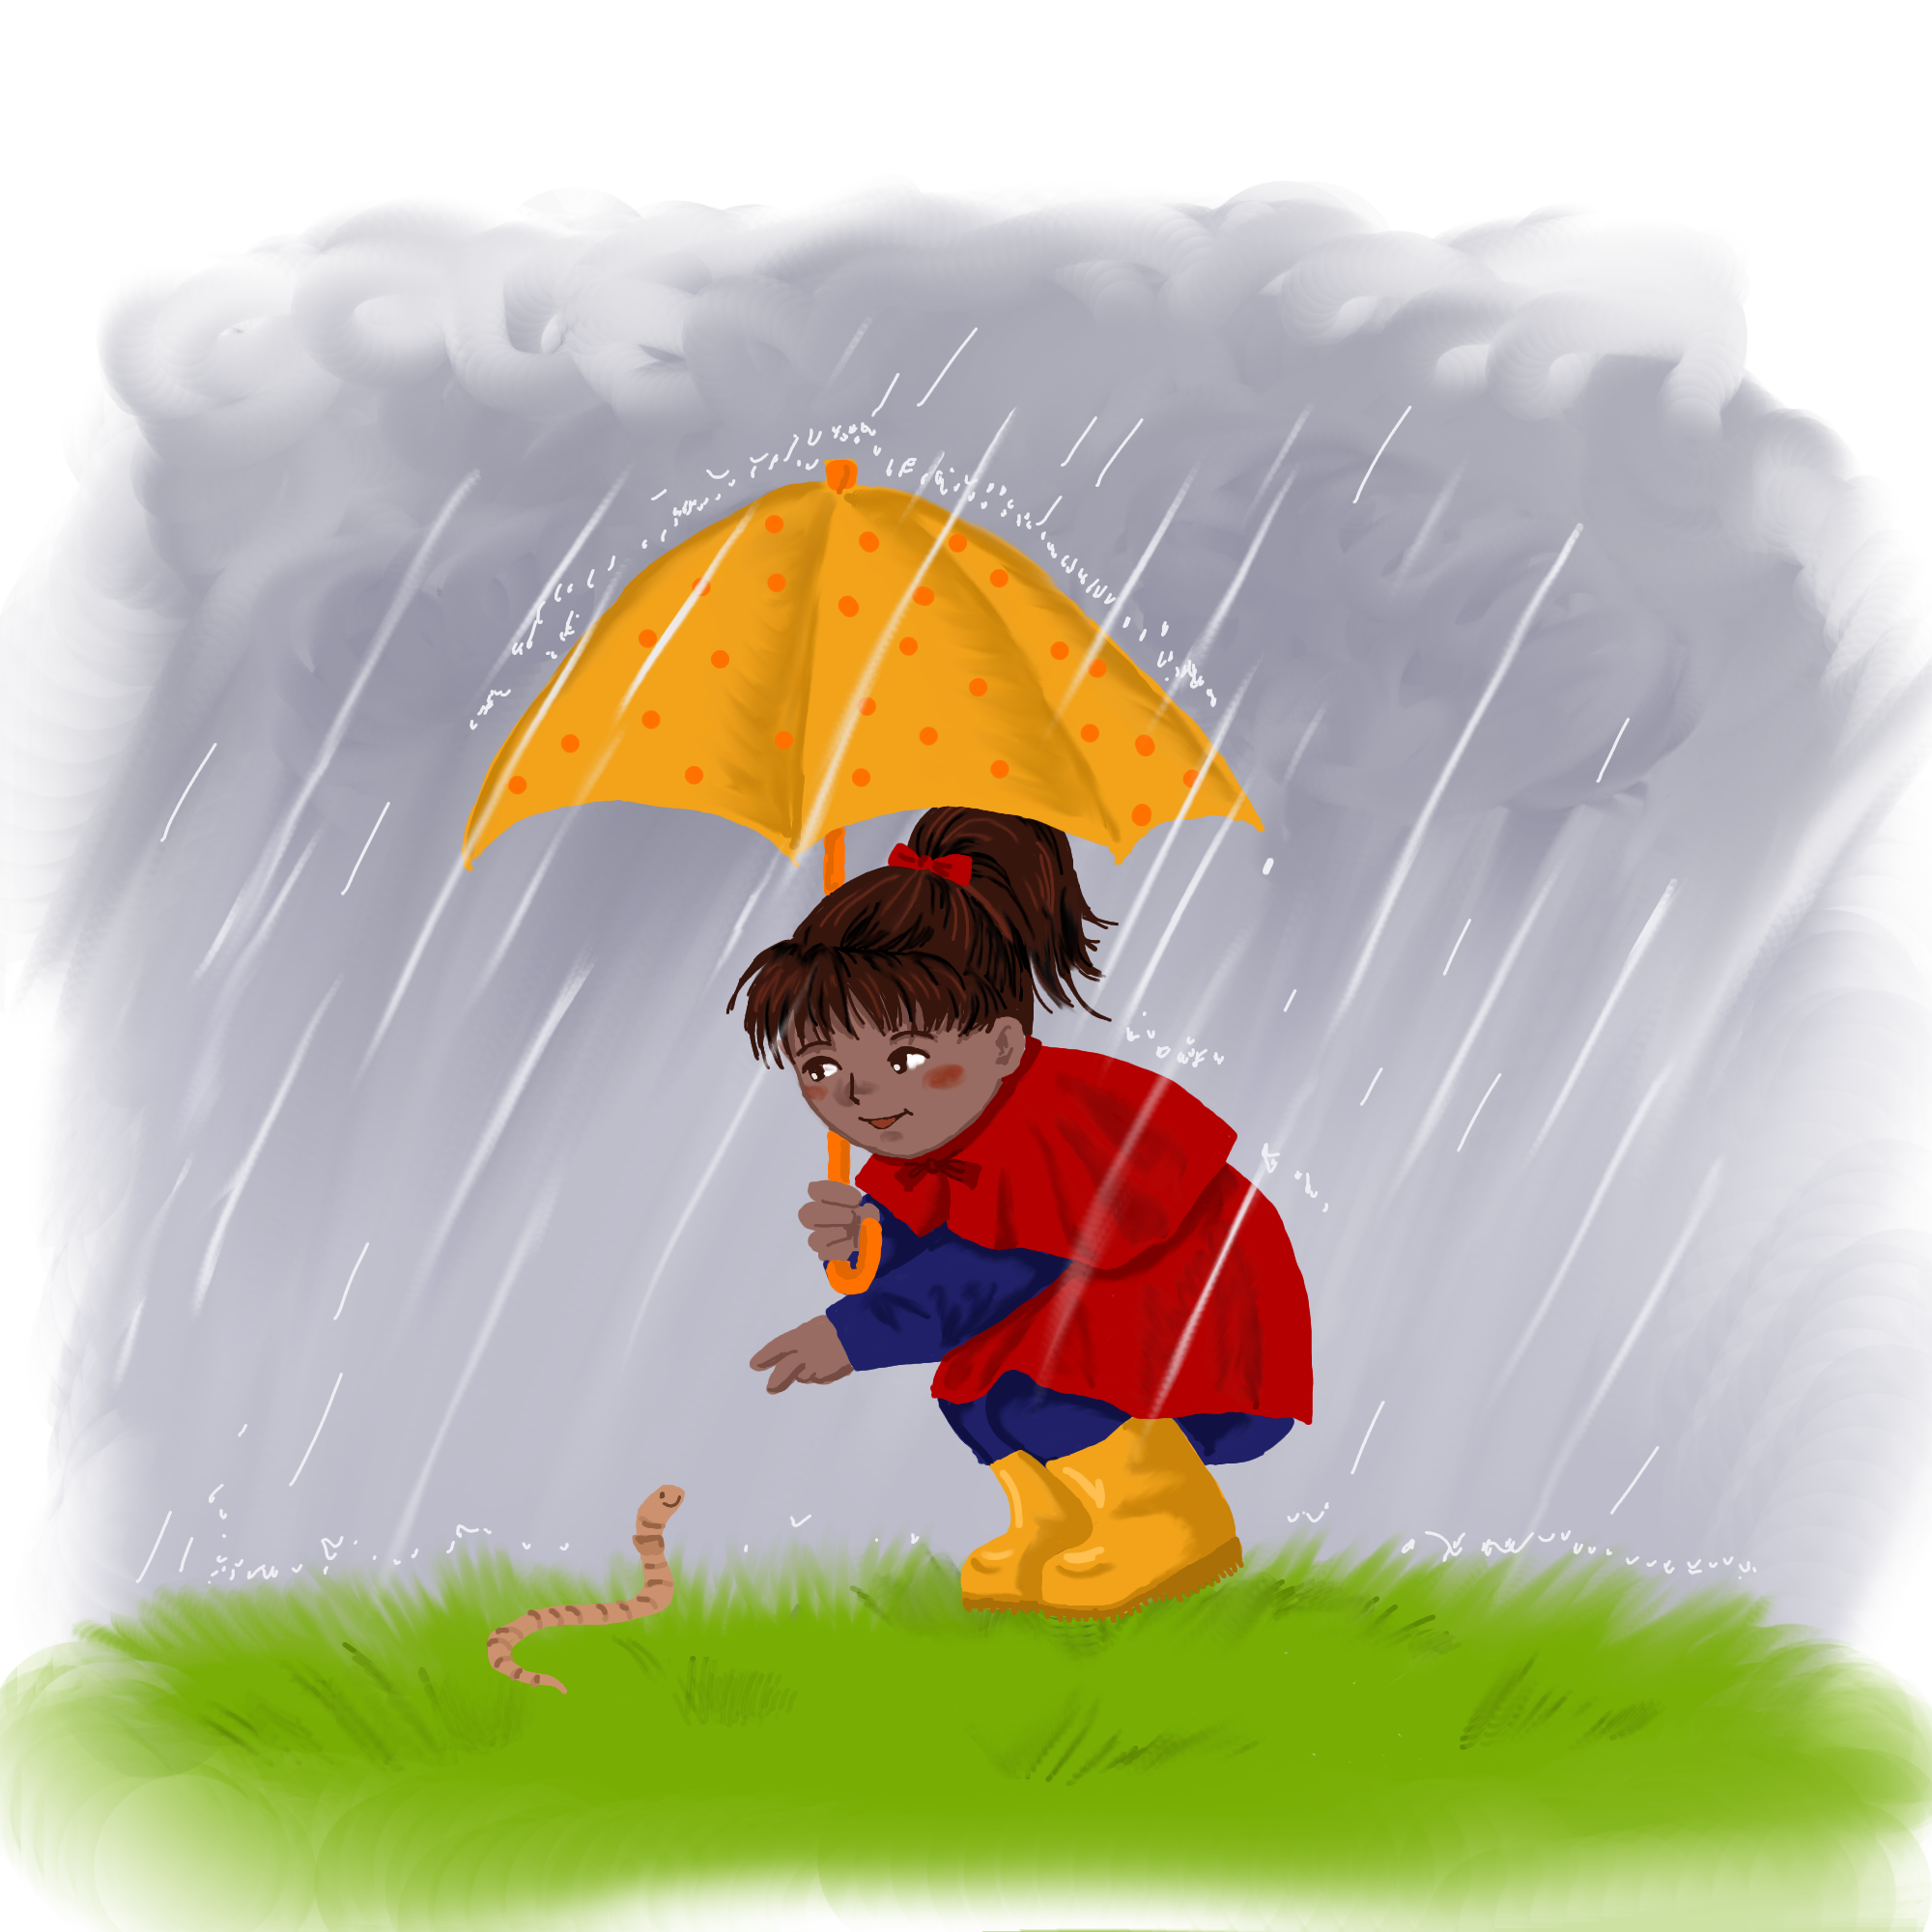
\includegraphics[scale = 0.1]{monty1.png}
\end{center}
}

\frame[t]{
\begin{center}
 
\includegraphics[scale=0.1]{aliens.png}
\end{center}
}

\frame[t]{
\begin{center}
 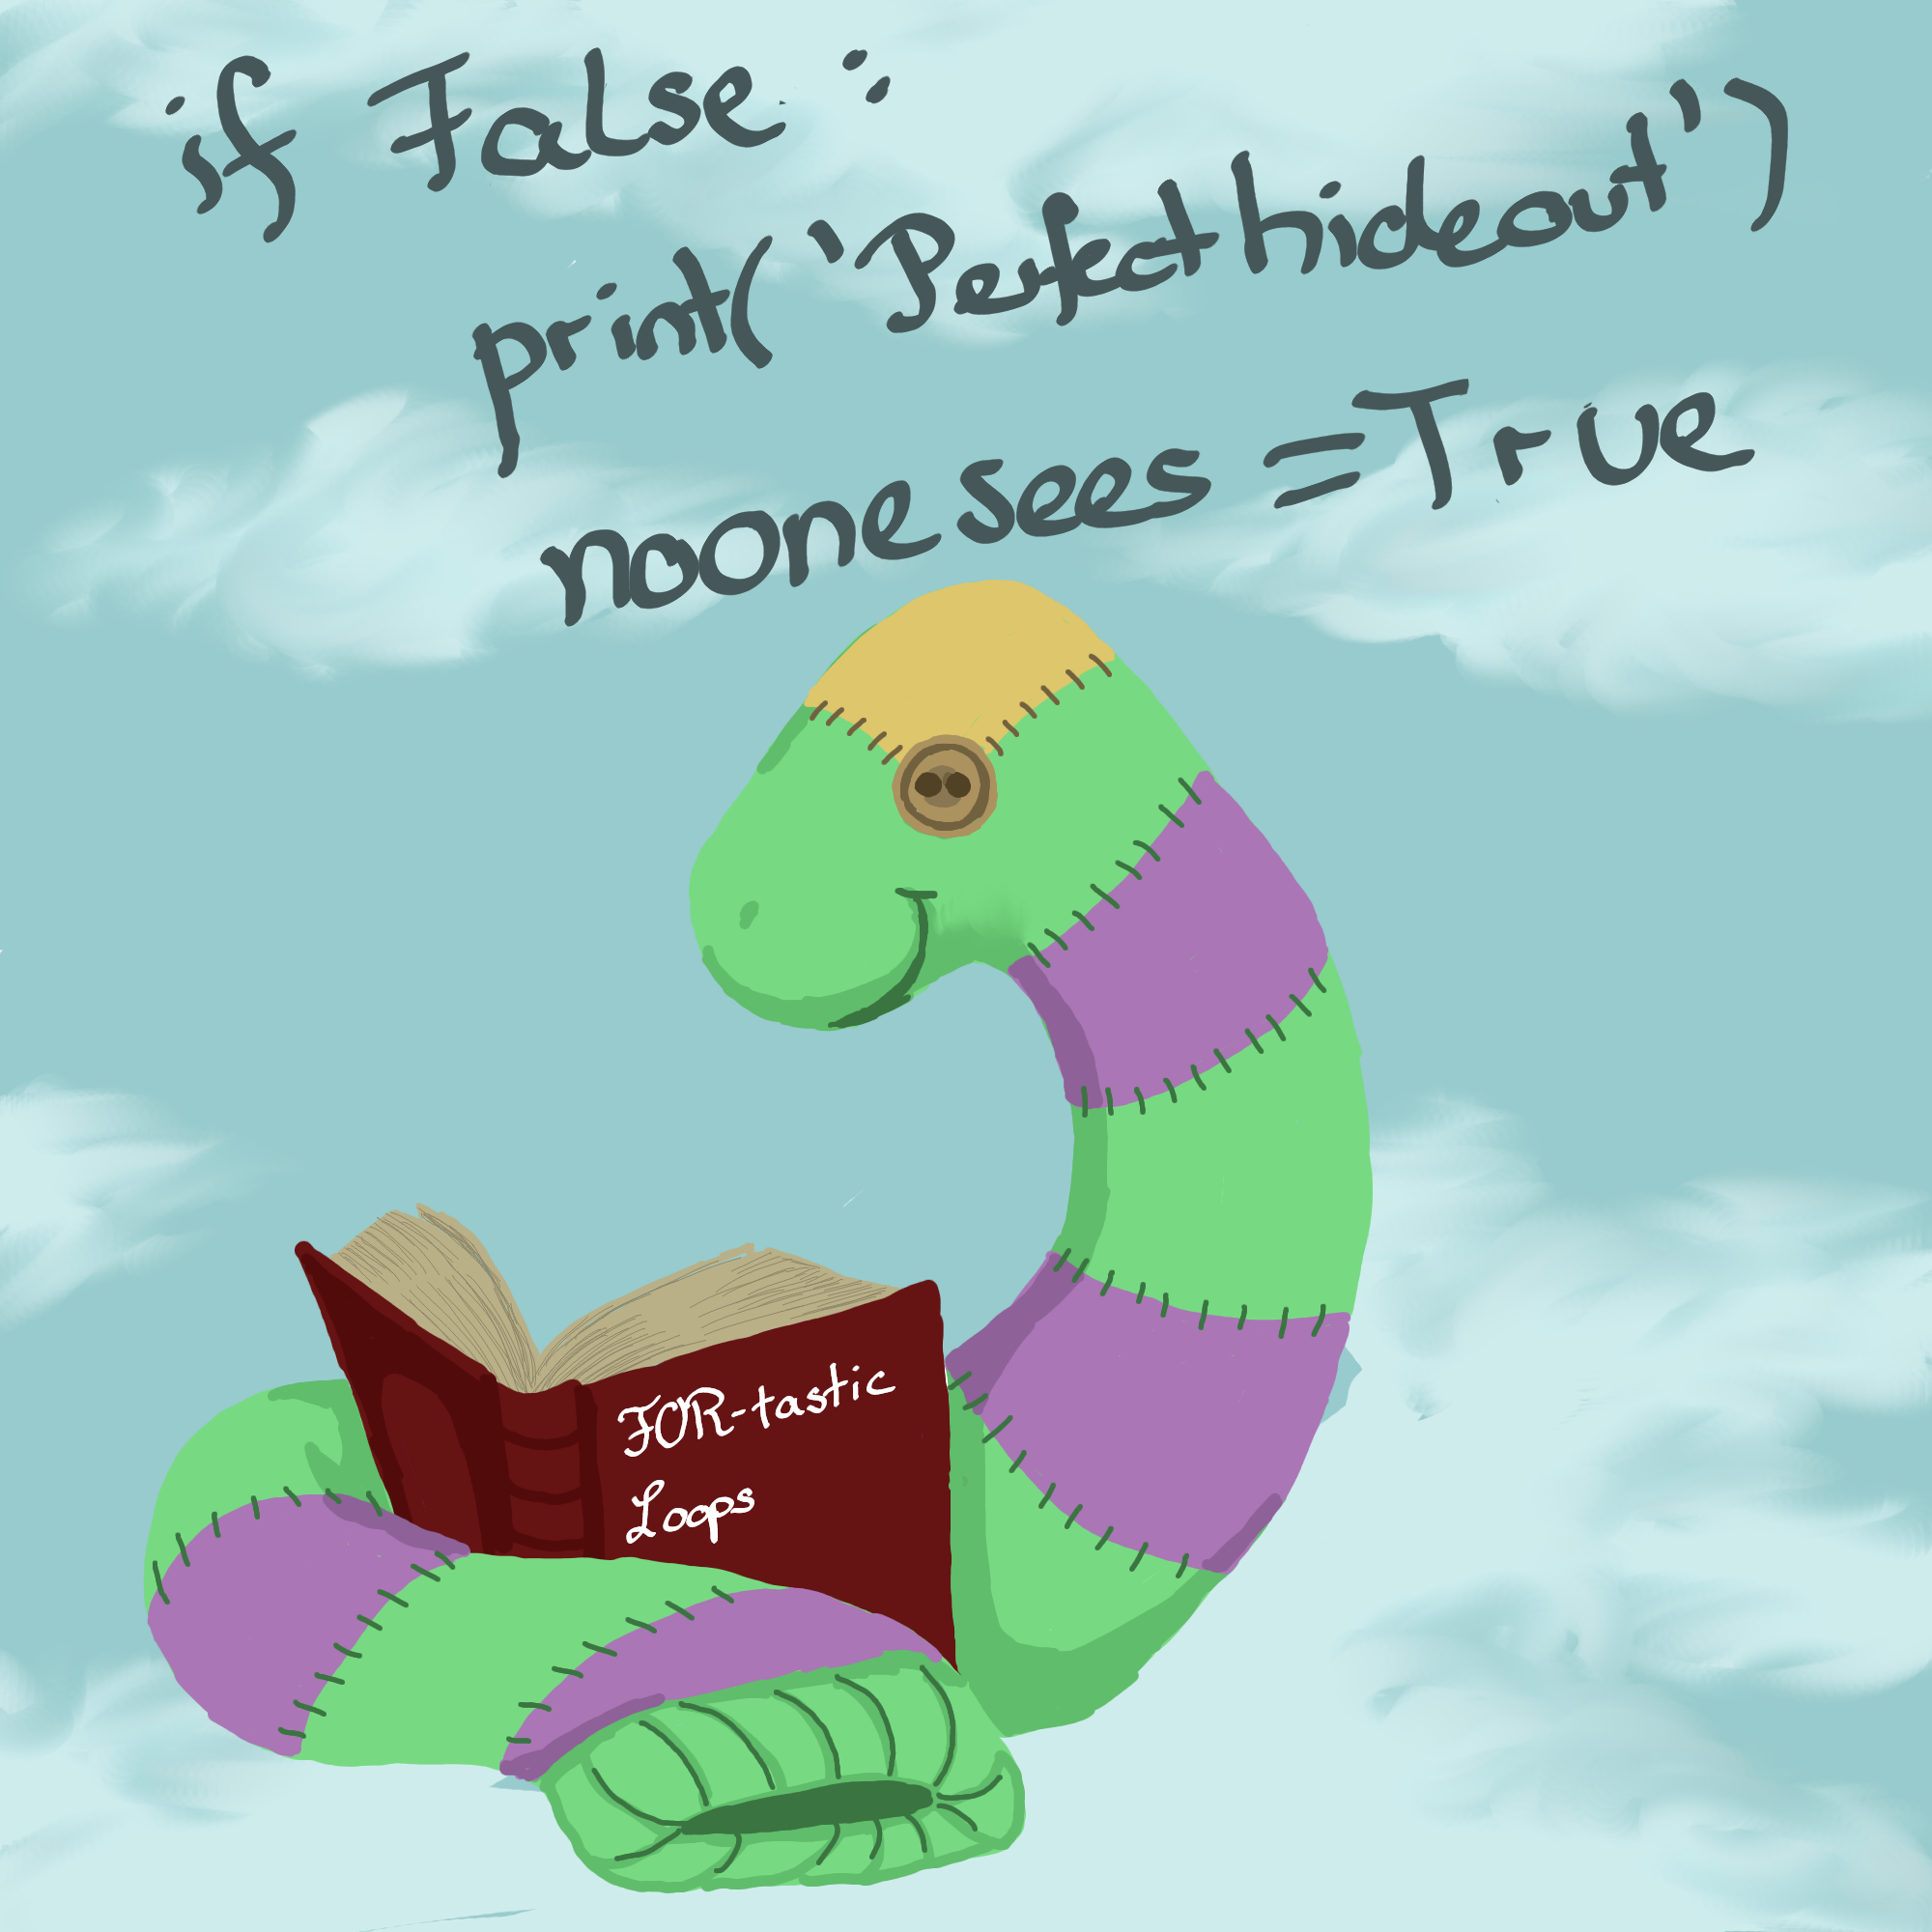
\includegraphics[scale=0.1]{py.png}
\end{center}
}





%%Kein Plan, ne?
%% Muss man gucken wegen python, was ich genau vorlesen will etc.
%%welchen teil lese ich? Evtl Code reinkopieren und zeigen während lesen



\frame[t]{\frametitle{}
\vspace*{2 cm}
\begin{block}{Variablenspiele}
 Meistere folgende Aufgaben:
 \begin{itemize}
  \item[a)] Erstelle die Variable \texttt{p} und weise ihr den Wert 3 zu.
  \item[b)] Erstelle die Variable \texttt{q} und weise ihr den Wert 12 zu.
  \item[c)] Berechne \texttt{q/p} und speichere das Ergebnis in der Variable \texttt{r}.
  \item[d)] Gib die Inhalte aller Variablen aus.
 \end{itemize}
\end{block}
 }


\frame[t]{\frametitle{}
\vspace*{2,7 cm}
\begin{block}{Die erste Pr\"ufung}
 Erstelle dir ebenfalls zwei Variablen \texttt{frosch} und \texttt{ente} und weise ihnen 
 verschiedene Werte zu, die du aussuchen kannst.
 Vertausche jetzt die Inhalte der beiden Variablen. Kannst du das?
\end{block}
}

\frame[t]{\frametitle{}
 \vspace*{3 cm}
 \begin{center}
  \Large{Skizzen auf GitHub: carinawi \\ https://github.com/carinawi}
 \end{center}
}

%Müssen wir evtl. hochladen
%Also sagen wir mal 40*4 Stunden brauche ich, Stundenlohn 25 Eur brutto
% also wären das 4000 Eur brutto. Das heisst also, ich kriege erstmal alles, bis die 4000 abbezahlt sind
% wenn man also wirklich 1 euro pro verkauf kriegt, müssten jetzt erstmal 4000 Leute das auch kaufen. 
% den gewinn überlass ich dann eben dem user oder will ne beteiligung von 50 % oder so...weiß nicht...


\end{document}